\documentclass[a4paper]{article}

\usepackage[utf8]{inputenc}
\usepackage[english]{babel}
\usepackage[round]{natbib}
% Additional packages
\usepackage[utf8]{inputenc}
\usepackage{subfig}
\usepackage[pdftex,pdfpagelabels,bookmarks,hyperindex,hyperfigures]{hyperref}
\hypersetup{%
   plainpages=false, 
   pdfpagelayout=SinglePage,
   bookmarksopen=false,
   bookmarksnumbered=true,
   breaklinks=true,
   linktocpage,
   colorlinks=true,
   linkcolor=blue,
   urlcolor=blue,
   citecolor=blue,
   anchorcolor=green
}      

% There seems to exist some kind of standard on using CHapter with capital.
\def\chapterautorefname{Chapter}

\newtheorem{algorithm}{Algorithm}

% Based on: http://lists.cs.princeton.edu/pipermail/topic-models/2010-December/001081.html
% http://www.mpi-inf.mpg.de/~dietz/probabilistic-models-tikz.zip
% by Laura Dietz (dietz at mpi-inf.mpg.de)
%
\usepackage{color}
\usepackage{array}
\usepackage{verbatim}
\usepackage{float}
\usepackage{amsmath}
\usepackage{amssymb}
\usepackage{esint}

%%%%%%%%%%%%%%%%%%%%%%%%%%%%%% LyX specific LaTeX commands.
%% Because html converters don't know tabularnewline
\providecommand{\tabularnewline}{\\}
\floatstyle{ruled}
\newfloat{algorithm}{tbp}{loa}[chapter]
\floatname{algorithm}{Algorithm}

%%%%%%%%%%%%%%%%%%%%%%%%%%%%%% Textclass specific LaTeX commands.
\usepackage{float}
\floatstyle{ruled}
\newfloat{algorithm}{tbp}{loa}
\floatname{algorithm}{Algorithm}
\newfloat{genmodel}{h}{loa}
\floatname{genmodel}{Generative Process}
\usepackage[noend]{algorithmic}
\newcommand{\forbody}[1]{ #1 \ENDFOR}
\newcommand{\ifbody}[1]{ #1  \ENDIF}
\newcommand{\whilebody}[1]{ #1  \ENDWHILE}
\renewcommand{\algorithmicprint}{\textbf{draw}}

%%%%%%%%%%%%%%%%%%%%%%%%%%%%%% User specified LaTeX commands.


\usepackage{euscript}

\DeclareSymbolFont{rsfscript}{OMS}{rsfs}{m}{n}
\DeclareSymbolFontAlphabet{\mathrsfs}{rsfscript}


% PDF formatting instructions for A4
\pdfpagewidth=210mm % for pdflatex
\pdfpageheight=296mm % for pdflatex


%%%%%%%% begin tikz %%%%%%
\usepackage{tikz,tkz-base}
\usetikzlibrary{shapes,decorations,shadows}
\usetikzlibrary{decorations.pathmorphing}
\usetikzlibrary{decorations.shapes}
\usetikzlibrary{fadings}
\usetikzlibrary{patterns}
\usetikzlibrary{calc}
\usetikzlibrary{decorations.text}
\usetikzlibrary{decorations.footprints}
\usetikzlibrary{decorations.fractals}
\usetikzlibrary{shapes.gates.logic.IEC}
\usetikzlibrary{shapes.gates.logic.US}
\usetikzlibrary{fit,chains}
\usetikzlibrary{positioning}
\usepgflibrary{shapes}
\usetikzlibrary{scopes}
\usetikzlibrary{arrows}
\usetikzlibrary{backgrounds}


\pgfdeclarelayer{background}
\pgfdeclarelayer{foreground}
\pgfsetlayers{background,main,foreground}

\tikzset{latent/.style={circle,fill=white,draw=red,thick,inner sep=1pt, 
minimum size=20pt, font=\fontsize{10}{10}\selectfont},
obs/.style={latent,fill=gray!25},
const/.style={rectangle, inner sep=0pt},
factor/.style={rectangle, fill=red,minimum size=7pt, inner sep=0pt},
yellow/.style={latent,minimum size=15pt,fill=yellow!75},
blue/.style={latent,minimum size=15pt,fill=blue!75},
-/.style={color=red, thick},
>={triangle 45}}




% shapename, fitlist, caption, pos
\newcommand{\plate}[4]{
\node (invis#1) [draw, transparent, inner sep=1pt,rectangle,fit=#2] {};
\node (capt#1) [ below left=0 pt of invis#1.south east, xshift=0pt,yshift=-9pt] {\raisebox{0pt}[0pt]{\footnotesize{#3}}};
\node (#1) [draw=black!50,thick,inner sep=3pt,rectangle,rounded corners,fit=(invis#1) (capt#1),#4] {};
}


\newcommand{\shiftedplate}[5]{
\node (invis#1) [draw, transparent, inner sep=0 pt,rectangle,fit=#2] {};
\node (capt#1) [#5, xshift=2pt] {\footnotesize{#3}};
\node (#1) [draw,inner sep=2pt, rectangle,fit=(invis#1) (capt#1),#4] {};
}

%shapename, pos, caption, in1, in2, out, captpos
\newcommand{\twofactor}[7]{
\node (#1) [factor] at #2 {};
\node (capt#1) [#7 of #1]{\footnotesize{#3}};
\draw [-] (#4) -- (#1) ;
\draw [-] (#5) -- (#1) ;
\draw [->,thick] (#1) -- (#6);
}

%shapename, pos, caption, in, out, captpos
\newcommand{\factor}[6]{
\node (#1) [factor] at #2 {};
\node (capt#1) [#6 of #1]{\footnotesize{#3}};
\draw [-] (#4) -- (#1) ;
\draw [->,thick] (#1) -- (#5);
}

% name, --, caption, pos
\newcommand{\nofactor}[4]{
\node (#1) [factor, #2]  {};
\node (capt#1) [#4 of #1]{\footnotesize{#3}};
}

%shapename,  fitlist, caption
\newcommand{\namedgate}[3]{
\node (invisgate#1) [rectangle, draw, transparent,  fit=#2] {};
\node (gatecapt#1) [ above right=0 pt of invisgate#1.north west, xshift=-1pt ] {\footnotesize{#3}};
\node (#1) [rectangle,draw,dashed, inner sep=2pt, fit=(invisgate#1)(gatecapt#1)]{};

}

%shapename,  fitlist, caption
\newcommand{\gate}[3]{
\node (#1) [rectangle,draw,dashed, inner sep=2pt, fit=#2]{};
}

%shapename,  fitlist1, fitlist2, caption1, caption2
\newcommand{\vertgate}[5]{
\node (invisgateleft#1) [rectangle, draw, transparent,  fit=#2] {};
\node (gatecaptleft#1) [ above left=0 pt of invisgateleft#1.north east, xshift=1pt ]{\footnotesize{#3}};
\node (invisgateright#1) [rectangle, draw, transparent,  fit=#4] {};
\node (gatecaptright#1) [ above right=0 pt of invisgateright#1.north west, xshift=-1pt ] {\footnotesize{#5}};
\node (#1) [rectangle,draw,dashed, inner sep=2pt, fit=(invisgateleft#1)(gatecaptleft#1)(invisgateright#1)(gatecaptright#1)]{};
\draw [-, dashed] (#1.north) -- (#1.south);
}


\newcommand{\vertgateSpec}[5]{
\node (invisgateleft#1) [rectangle, draw, transparent,  fit=#2] {};
\node (gatecaptleft#1) [ above left=0 pt of invisgateleft#1.north east, xshift=1pt ]{\footnotesize{#3}};
\node (invisgateright#1) [rectangle, draw, transparent,  fit=#4] {};
\node (gatecaptright#1) [ above right=0 pt of invisgateright#1.north west, xshift=-1pt ] {\footnotesize{#5}};
\node (#1) [rectangle,draw,dashed, inner sep=2pt, fit=(invisgateleft#1)(gatecaptleft#1)(invisgateright#1)(gatecaptright#1)]{};
\draw [-, dashed] (#1.70) -- (#1.290);
}

\newcommand{\horgate}[5]{
\node (invisgateleft#1) [rectangle, draw, transparent,  fit=#2] {};
\node (gatecaptleft#1) [ above right=0 pt of invisgateleft#1.south west, xshift=1pt ]{\footnotesize{#3}};
\node (invisgateright#1) [rectangle, draw, transparent,  fit=#4] {};
\node (gatecaptright#1) [ below right=0 pt of invisgateright#1.north west, xshift=-1pt ] {\footnotesize{#5}};
\node (#1) [rectangle,draw,dashed, inner sep=2pt, fit=(invisgateleft#1)(gatecaptleft#1)(invisgateright#1)(gatecaptright#1)]{};
\draw [-, dashed] (#1.west) -- (#1.east);
}

\newcommand{\horogate}[5]{
\node (invisgateleft#1) [rectangle, draw, transparent,  fit=#2] {};
\node (invisgateright#1) [rectangle, draw, transparent,  fit=#4] {};
\node (#1) [rectangle,draw,dashed, inner sep=2pt, fit=(invisgateleft#1)(invisgateright#1)]{};
\node (gatecaptleft#1) [ above right=0 pt of #1.west, xshift=0pt ]{\footnotesize{#3}};
\node (gatecaptright#1) [ below right=0 pt of #1.west, xshift=0pt ] {\footnotesize{#5}};

\draw [-, dashed] (#1.west) -- (#1.east);
}


\newcommand{\vertogate}[5]{
\node (invisgateleft#1) [rectangle, draw, transparent,  fit=#2] {};
\node (invisgateright#1) [rectangle, draw, transparent,  fit=#4] {};
\node (#1) [rectangle,draw,dashed, inner sep=2pt, fit=(invisgateleft#1)(invisgateright#1)]{};
\node (gatecaptleft#1) [ below left=0 pt of #1.north, xshift=0pt ]{\footnotesize{#3}};
\node (gatecaptright#1) [ below right=0 pt of #1.north, xshift=0pt ] {\footnotesize{#5}};

\draw [-, dashed] (#1.north) -- (#1.south);
}



\title{Notes on Semi-Supervised `Novelty Detection'}
\author{André Susano Pinto}

\begin{document}
\maketitle

\section{Introduction}
The case presented here assumes that a machine learning system besides having access to samples of the known class also has access to unlabelled data representative of the whole world.
This may happen in some machine learning problems where a set of samples from a given class has been grouped and identified and although its possible to gather new samples its infeasible to classify them (eg.: the human classifier got bored)\footnote{Other examples of situations are given on \autoref{sec:detection}.}.

Under that assumption its possible to model the functions $P(x|know)$ and $P(x)$ representing both a conditional and an unconditional density function for a given input.
Using those its possible to define a threshold function for novelty detection as seen on \autoref{sec:threshold}.

In \autoref{sec:threshold-analysis} the described threshold is analyzed in more detail, and in \autoref{sec:experiment} experiments to test the described methods are presented.

\subsection{(Novelty?) Detection}
\note{I believe calling \emph{novelty detection} to the threshold described here is incorrect.
I am not sure which would be the correct term.}

This new assumption of access to unlabelled data makes it dubious whether it can still be classified as a \emph{novelty detection} problem:
\begin{quotation}
`Novelty detection is the identification of new or unknown data or signal that a machine learning system is not aware of during training.' - \cite{markou2003novelty}.
\end{quotation}

But it is also different from a binary classification problem since instead of negative samples there is access to unlabelled data\footnote{Though several detection systems use binary classification techniques where negative samples are obtained by randomly sampling.}.


%%%%%%%%%%%%%%%%%%%%%%%%%%%%%%%%%%%%%%%%%%%%%%%%%%%%%%%%%%%%%%%%%%%%%%%%%%%%%%%%%
%%%%%%%%%%%%%%%%%%%%%%%%%%%%%%%%%%%%%%%%%%%%%%%%%%%%%%%%%%%%%%%%%%%%%%%%%%%%%%%%%
%%%%%%%%%%%%%%%%%%%%%%%%%%%%%%%%%%%%%%%%%%%%%%%%%%%%%%%%%%%%%%%%%%%%%%%%%%%%%%%%%
\section{Concept Detection}
\label{sec:detection}

\note{
This lacks literature background, and writing it on an airplane does not helps.
Gotta find some papers on the subject
}

In several machine learning problems the target is to detect whether a concept is present.
(eg.: face detection, intrusion detection).

In cases where negative samples are \emph{abundant} (face detection, music/speech detection), systems often use a random sample of input space to represent negative samples and then perform detection using a normal 2-class classification.

On systems where negative samples are very rare (intrusion-detection, cancer-detection), system need to use other approaches based on novelty detection\dots

Some cases lie somewhere in between: negative samples are easy to obtain, but they are not that common that we can assume a random sample does not contains positive samples in it. Hence we cannot treat a random sample as a negative.

In those cases we point to the usage of the ratio between conditional and unconditional probabilities as a detection function.
Examples of cases where this type of detection is may or may not appear are given below:

\subsubsection*{Unconstrainted labelled data}
On a system where a user is asked to tag samples with words representing concepts it is fairly easy to filter positive samples for a given concept.
Although getting negative samples is an impossible task, as the non-presence of a given tag on a sample does not necessarily makes that a negative sample for the concept.

Eg.: associating concepts with images, tagging objects on images, ...

\subsubsection*{Tag-prediction systems}
Music, image, text, news, auto-tagging\dots

\subsubsection*{Good approximation of density functions}
A good approximation of probability functions for a given input is necessary for the performance of the presented method.
So its expected to have uses where the input space is small or it can be modelled with some precision (eg.: independent features).


%%%%%%%%%%%%%%%%%%%%%%%%%%%%%%%%%%%%%%%%%%%%%%%%%%%%%%%%%%%%%%%%%%%%%%%%%%%%%%%%%
%%%%%%%%%%%%%%%%%%%%%%%%%%%%%%%%%%%%%%%%%%%%%%%%%%%%%%%%%%%%%%%%%%%%%%%%%%%%%%%%%
%%%%%%%%%%%%%%%%%%%%%%%%%%%%%%%%%%%%%%%%%%%%%%%%%%%%%%%%%%%%%%%%%%%%%%%%%%%%%%%%%
\section{Threshold}
\label{sec:threshold}

The threshold is based on the probability that a given concept is present on a sample
knowing both that the concept samples and the unlabelled samples come from the same distribution $P$.

In that case our optimal threshold would be:
$P(concept | x) > 1/2$, which means we assume the concept is present if we have more than chance probability of getting it right.

Using bayes rules we obtain:

\begin{equation}\frac{P(x|concept) P(concept)}{P(x)} > \frac{1}{2}\end{equation}
\begin{equation}\frac{P(x|concept)}{P(x)} > \frac{1}{2 P(concept)}\end{equation}
\begin{equation}\frac{P(x|concept)}{P(x)} > K_{threshold}\end{equation}

\note{Novelty detection techniques often assume a constant $P(x)$ and then threshold is performed only on the conditional probability density function.}

Proposed detection method:
\begin{itemize}
\item From the environment draw labelled and unlabelled samples.
\item From those learn both $P(x|class \in known)$ and $P(x)$.
\item Define a detection threshold based on $P(x|class \in known)/P(x)$.
\end{itemize}


%%%%%%%%%%%%%%%%%%%%%%%%%%%%%%%%%%%%%%%%%%%%%%%%%%%%%%%%%%%%%%%%%%%%%%%%%%%%%%%%%
%%%%%%%%%%%%%%%%%%%%%%%%%%%%%%%%%%%%%%%%%%%%%%%%%%%%%%%%%%%%%%%%%%%%%%%%%%%%%%%%%
%%%%%%%%%%%%%%%%%%%%%%%%%%%%%%%%%%%%%%%%%%%%%%%%%%%%%%%%%%%%%%%%%%%%%%%%%%%%%%%%%
\clearpage
\section{Threshold Analysis}
\label{sec:threshold-analysis}

\subsection{Bounding $P(c)$}
\note{This was just a random though... if we can bound $P(c)$ in some way then we get
      some information on how sure we are about a decision. Though its only possible
      to bound it from above, and even that not sure if its computational feasible.}

\begin{equation}P(x) = \sum_{c}^{} P(x|c) P(c)\end{equation}
\begin{equation}0 \le P(x|c) P(c) \le P(x)\end{equation}
\begin{equation}0 \le P(c) \le \frac{P(x)}{P(x|c)}\end{equation}


\subsection{What does a ROC curve looks like for an optimal detector}
\note{The ROC curve shape shows if a detector is perfect given an input space.
      I guess somewhere there should be literature reference to such a simple concept}

Proof would be something like:

An element of the input space is responsible for a vector change of $(TP, FP)$ in the ROC
curve.
A threshold functions orders the input space.
And the best is to take the greedy approach of sorting the input by $TP/FP$.
That is equivalent to a convex ROC curve.

This leads to the important property:
\emph{whatever threshold function you use,
if you get a convex ROC curve, there is no way to perform better using that input space.}

At the same time we can proof an ordering on $TP/FP$ to be the same as $TP/(FP+TP)$.
Which is coherent with the threshold of: $P(x|concept)/P(x)$.

%%%%%%%%%%%%%%%%%%%%%%%%%%%%%%%%%%%%%%%%%%%%%%%%%%%%%%%%%%%%%%%%%%%%%%%%%%%%%%%%%
%%%%%%%%%%%%%%%%%%%%%%%%%%%%%%%%%%%%%%%%%%%%%%%%%%%%%%%%%%%%%%%%%%%%%%%%%%%%%%%%%
%%%%%%%%%%%%%%%%%%%%%%%%%%%%%%%%%%%%%%%%%%%%%%%%%%%%%%%%%%%%%%%%%%%%%%%%%%%%%%%%%
\clearpage
\section{Evaluation and Experiments}
\label{sec:experiment}

This section describes the two experiences that were run to evaluate the methods.
\begin{description}
\item[\autoref{sec:simple-experiment}] presents a toy experience that aims at
  showing the importance of using $P(x)$ to estimate a novelty threshold and
  it importance when dealing with features that have a tendency to be highly
  biased such as the semantic data used on our sample.

\item[\autoref{sec:dora-experiment}] runs comparisons of the presented threshold
  on a real-world scenario, where a robot has to identify room categories based
  on obtained semantic data, such as object presence and room size.
  The experiment is run both with a fictitious distribution and with a real world
  dataset.
\end{description}

Other possible experiences are:
\begin{itemize}
\item run this type of classification on datasets such as \emph{LabelMe} databases,
  either by using user-supplied tags as semantic data or by extracting them with some
  image analysis.
\end{itemize}


\subsection{Simple}\label{sec:simple-experiment}
For a better understanding of how the knowledge of the unconditional probability $P(x)$ can help to improve the detection threshold
a very small toy experiment was run:

Using a simple distribution, described in \autoref{tab:simple-distribution},
labelled ($known = \{kitchen, corridor\}$)
and unlabelled samples where drawn.
$P(x|class \in known)$ and $P(x)$ where then approximated using simple accumulation tables
(only 6 different inputs).
The input space was then sorted according to the presented thresholds obtaining
the results as seen on \autoref{tab:simple-data-sorted}.

\begin{table}[hb]
\begin{center}
\input{simple-data/explain}
\end{center}
\caption{\label{tab:simple-distribution}Distribution used on the simple experiment. Each column cell shows $P(feature|class)$}
\end{table}

\begin{table}
\centering
\subfloat[Input space sorted by threshold $P(x|class \in known)$]{\input{simple-data/density_threshold}}
\qquad
\subfloat[Input space sorted by threshold $P(x|class \in known)/P(x)$]{\input{simple-data/semi_threshold}}
\caption{\label{tab:simple-data-sorted}Input space sorted by threshold functions.}
\end{table}

The results obtained demonstrate that using the conditional probability function
as a novelty threshold leads to poor performance: it classified (corridor,square) as
the most novel case.
This happens because the likelihood of such a sample is very low.
Nonetheless when using the factor $P(x)$ the system is able to take in consideration
that the low probability of that sample on the labelled data arrives from the low
probability of finding such a sample and not necessarily from a novel case.


\clearpage
\subsection{Dora with world model}
\label{sec:dora-experiment}



This experience is similar to the simple experiment run in \autoref{sec:simple-experiment}.
But this time using a more realistic distribution (\autoref{tab:dora-world-distribution}) with
11 different room categories and with a feature space containing semantic data for:
room size, room shape, visual appearance and 6 different objects.

Having perfect information of the distributions $P(x|c \in known)$ and $P(x)$
allows us to build an optimal detector as seen on \autoref{fig:dora-data-perfect}.

\begin{figure}[h]
\centering
\includegraphics[width=0.75\textwidth]{dora-data/roc-perfect.pdf}
\caption{ROC curve for thresholds based on perfect information running on the dora distribution.
         The convex curve for $P(x|k)/P(x)$ shows its optimal.}
\label{fig:dora-data-perfect}
\end{figure}

Nonetheless to build that optimal detector we need information on $P(x)$ which often is not available.
We focus then on the study of the bias introduced by only using $P(x|k)$ as a threshold.

For that we compared all roc curves based on perfect information for each missing
classes (\autoref{fig:roc-curves-missing-1}).

\begin{figure}[h]
 \centering
 \subfloat[Anteroom]{\includegraphics[width=0.33\textwidth]{dora-data/roc-missing-anteroom.pdf}}
 \subfloat[Bathroom]{\includegraphics[width=0.33\textwidth]{dora-data/roc-missing-bathroom.pdf}}
 \subfloat[Computer Lab]{\includegraphics[width=0.33\textwidth]{dora-data/roc-missing-computerlab.pdf}} \\
 \subfloat[Conference Hall]{\includegraphics[width=0.33\textwidth]{dora-data/roc-missing-conferencehall.pdf}}
 \subfloat[Double Office]{\includegraphics[width=0.33\textwidth]{dora-data/roc-missing-doubleoffice.pdf}}
 \subfloat[Hallway]{\includegraphics[width=0.33\textwidth]{dora-data/roc-missing-hallway.pdf}} \\
 \subfloat[Kitchen]{\includegraphics[width=0.33\textwidth]{dora-data/roc-missing-kitchen.pdf}}
 \subfloat[Meeting Room]{\includegraphics[width=0.33\textwidth]{dora-data/roc-missing-meetingroom.pdf}}
 \subfloat[Professors Office]{\includegraphics[width=0.33\textwidth]{dora-data/roc-missing-professorsoffice.pdf}} \\
 \subfloat[Robot Lab]{\includegraphics[width=0.33\textwidth]{dora-data/roc-missing-robotlab.pdf}}
 \subfloat[Single Office]{\includegraphics[width=0.33\textwidth]{dora-data/roc-missing-singleoffice.pdf}}

\caption{\label{fig:roc-curves-missing-1}ROC curves for all one single missing category in the known data.}
\end{figure}

\begin{figure}
\centering
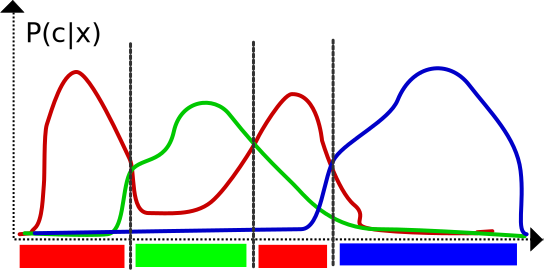
\includegraphics[width=0.75\textwidth]{dora-data/classification.pdf}
\caption{\label{fig:confusion-matrix-dora}
         Confusion matrix for the 11 classes that make up the dora distribution.}
\end{figure}

That was lead by the fact conditional density threshold gives very poor results on detecting classes
that are easily confused with other classes using the given feature space (see confusion matrix in
\autoref{fig:confusion-matrix-dora}).
As the lack of knowledge of $P(x)$ limits the ability of the detector to correctly sort the feature
space to in a way that a bigger value is given to the inputs where the probability of being correct is more accurate.

Depending on the feature space used, this might be a very important property.
As it will greatly impact a novelty detector. For the case of semantic data used in dora:
very small feature spaces and lack of specific features to detect some room categories.

For that we implemented a very simple approach to unconditional density probability and compared the results
\dots

\begin{sidewaystable}[h]
\begin{center}
\scalebox{0.50}{\input{dora-data/explain}}
\end{center}
\caption{\label{tab:dora-world-distribution}World model used in Dora. Each column cell shows $P(feature|class)$}
\end{sidewaystable}


\clearpage
\subsection{Modeling the World with Graphical Models}
The previous experiences assume perfect knowledge on the probability distributions functions.
This sections presents how Dora models those distributions and how to perform novelty detection with them.

Dora uses \emph{probabilistic graphical models} to represent all extracted knowledge from the world.
Those allow to easily model certain probabilistic properties such as conditional independence
and easy the process of several computational problems on the distributions.
Several tools exists for this type of graphical manipulation such as: \emph{Bayesian networks}, \emph{Markov Random Fields}
or \emph{Factor Graphs}.

Dora underlying graphical methods are based on \emph{Factor Graphs}\citep{kschischang2001factor}: bipartites graphs composed of variable and factor nodes representing the random variables and several factor functions between the variables that are used to decomposed the distribution.


\begin{figure}[h]
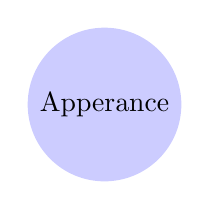
\begin{tikzpicture}
\node[circle,fill=blue!20] (room1) {Room};
\node[circle,fill=blue!20] (Appearance) {Apperance};
\end{tikzpicture}
\caption{Example of a factor graph used for Dora.}
\end{figure}


At any moment dora has a graph $G$ representing a set of random variables the system is aware of and all the probabilistic connections between them.
The observed values are set by the sensed properties and inferences can be done on the remaining ones.

Assuming the graph edges capture the properties of the distribution $P(x|known)$.
$G$ becomes indeed our replacement for that distribution and so $P(x|known) = P(x|G)$.

In order to generate a simple and interesting properties we decided to model $P(x)$ also with a graphical model.



Evaluating $P(x|G)/P(x|G')$...


Method:
\begin{enumerate}
\item Train a graph model for unlabelled data without the labelled variables.
\item Add the labelled variables and train the factors with the labelled data.
\item Use $P(x|G)$ as novelty threshold.
\end{enumerate}

Comparison of the estimated models with respect to the perfect information functions as been done on
\autoref{fig:dora-data-simple}.
Important to notice that our model of unconditional probability is very simple, still is able to improve
our novelty detection.

\note{Describe better which approach we used to model $P(G)/P(G')$}
\note{Perform experience with real data}


\note{The graphics are a bit "cheated", since theres an added epsilon on the returned value
      so the probabilities functions do not return 0. This is because at the moment if on the known
      samples we never see a given value we don't know it belongs to the possible feature space.
      Has to be corrected.}

\begin{figure}[h]
\centering
\includegraphics[width=\textwidth]{dora-data/roc-simple.pdf}
\caption{ROC curve for thresholds learned on samples from samples in the dora distribution}
\label{fig:dora-data-simple}
\end{figure}

\note{The graphics are a bit "cheated", since theres an added epsilon on the returned value
      so the probabilities functions do not return 0. This is because at the moment if on the known
      samples we never see a given value we don't know it belongs to the possible feature space.
      Has to be corrected.}





\clearpage
\subsection{How Dora models the world?}
\label{sec:dora-models}

Currently dora uses a \emph{probabilistic graphical model} to model the world.
All variables that the system see are added and connected in between with the
\emph{probabilistic factors} that the system is aware of.
Those factors are learned from the labelled data that the system is given when
training.

The proposal here is to also use such an approach to model the unconditional
probability.
Under that a novelty detection threshold can be easily implemented
reusing the \emph{probabilistic graphical model} $G$ that dora uses as
representation of the world:
\begin{description}
\item[$P(x|know)$] is obtained evaluating $P(G)$.
\item[$P(x)$] can be obtained by creating $G'$ as an instance of $G$ but with the
variable node we want to perform novelty detection removed and the factors associated
with it replaced with factors learned from the unlabelled data.
\end{description}

We point to an additional simplification that if the original graphical model factors
depending on the variable to perform novelty detection were previously split on a
conditional and unconditional factors. Then $G'$ could be obtained by simply removing
all the factors associated with the variable to perform novelty detection on.


%%%%%%%%%%%%%%%%%%%%%%%%%%%%%%%%%%%%%%%%%%%%%%%%%%%%%%%%%%%%%%%%%%%%%%%%%%%%%%%%%
%%%%%%%%%%%%%%%%%%%%%%%%%%%%%%%%%%%%%%%%%%%%%%%%%%%%%%%%%%%%%%%%%%%%%%%%%%%%%%%%%
%%%%%%%%%%%%%%%%%%%%%%%%%%%%%%%%%%%%%%%%%%%%%%%%%%%%%%%%%%%%%%%%%%%%%%%%%%%%%%%%%
\cleardoublepage
\phantomsection
\addcontentsline{toc}{section}{References}

\bibliographystyle{plainnat}
\bibliography{refs}

\end{document}

